% !TEX program = xelatex
% !TEX root = main.tex
\documentclass[12pt, a4paper]{article}

% --- PACOTES ---
% Essenciais e de Idioma
\usepackage[brazilian]{babel}
\usepackage{fontspec}

% Layout e Geometria
\usepackage[margin=2.5cm]{geometry}
\usepackage{fancyhdr}
\usepackage{titlesec}
\usepackage{titling}
\usepackage{authblk}

% Matemática e Física
\usepackage{amsmath,amssymb,amsfonts,mathtools,amsthm}
\usepackage{physics}               % Comandos como \dd, \grad, \vb, etc.
\usepackage{tensor}                % Para tensores com índices
\usepackage{bm}                    % Símbolos matemáticos em negrito
\usepackage{cancel}                % Para cortar expressões matemáticas

% Referências e Links
\usepackage{hyperref}
\usepackage{cleveref}              % Referências inteligentes (\cref{...})
\usepackage{bookmark}              % Melhora os bookmarks do PDF

% Bibliografia e Citações
\usepackage{csquotes}              % Necessário para alguns estilos do biblatex
\usepackage[backend=biber, style=numeric-comp, sorting=none]{biblatex}


% Visual
\usepackage{graphicx}
\usepackage{gensymb}
\usepackage{xcolor}
\usepackage{enumitem}              % Controle avançado de listas
\usepackage{footnote}
\usepackage{manyfoot}              % Múltiplos tipos de notas de rodapé
\usepackage{tocloft}               % Para customizar o sumário
\usepackage{lipsum}                % Apenas para texto de exemplo
\usepackage{comment}               % Serve pra comentar blocos inteiros



% --- AMBIENTES ---
\newtheoremstyle{meuremarkstyle} % <name>
  {\topsep}                   % <space above>
  {\topsep}                   % <space below>
  {\normalfont}               % <body font> - texto normal para o conteúdo
  {}                          % <indent amount>
  {\itshape}                 % <head font> - italico para o título
  {:}                         % <head punctuation> - AQUI ESTÁ O SEGREDO: dois pontos!
  {.5em}                      % <space after head>
  {\underline{\thmname{#1}}}  % <head spec> - deixar vazio para o padrão
\theoremstyle{meuremarkstyle}
\newtheorem*{notação}{Notação}

\newtheoremstyle{definicao} % <name>
  {\topsep}                   % <space above>
  {\topsep}                   % <space below>
  {\normalfont}               % <body font> - texto normal para o conteúdo
  {}                          % <indent amount>
  {\itshape}                 % <head font> - italico para o título
  {:}                         % <head punctuation> - AQUI ESTÁ O SEGREDO: dois pontos!
  {.5em}                      % <space after head>
  {\underline{\thmname{#1}}}  % <head spec> - deixar vazio para o padrão
\theoremstyle{definicao}
\newtheorem*{definição}{Definição}



% --- CONFIGURAÇÃO DA BIBLIOGRAFIA ---
\addbibresource{referencias.bib}

% --- CONFIGURAÇÕES VISUAIS ---
% Parágrafos (sem indentação, com espaçamento)
\setlength{\parskip}{0.5em}
\setlength{\parindent}{0pt}

% Fonte Principal
\setmainfont{Latin Modern Roman} % Fonte padrão moderna, segura e completa

% Cabeçalho e Rodapé (Fancyhdr)
\pagestyle{fancy}
\fancyhf{} % Limpa todos os campos do cabeçalho e rodapé
\fancyhead[L]{\nouppercase{\leftmark}} % Esquerda: Seção atual (sem caixa alta)
\fancyhead[R]{\thepage}                 % Direita: Número da página
\renewcommand{\headrulewidth}{0.4pt}
\renewcommand{\sectionmark}[1]{\markboth{#1}{}}


% Formato dos Títulos (Titlesec)
\titleformat{\section}{\large\bfseries}{\thesection.}{1em}{}
\titleformat{\subsection}{\normalsize\bfseries}{\thesubsection}{1em}{}
\titleformat{name=\section, numberless}
  {\large\bfseries\centering}
  {}
  {0pt}
  {}

% Sumário Pontilhado (Tocloft)
\renewcommand{\cftsecleader}{\cftdotfill{\cftdotsep}}

% Notas de Rodapé (Manyfoot)
\DeclareNewFootnote{B}[fnsymbol]

% Configurações de Links (Hyperref)
\hypersetup{
    colorlinks=false,
    linkcolor=blue,
    citecolor=red,
    urlcolor=magenta,
    pdftitle={Título do Trabalho Final},
    pdfauthor={Primeiro Autor; Segundo Autor}, % Autores no metadata do PDF
}

% %%%%%%%%%%%%%%%%%%%%%%%%%%%%%%%%%%%%%%%%%%%%%%%%%%%%%%%
%                         DOCUMENTO
% %%%%%%%%%%%%%%%%%%%%%%%%%%%%%%%%%%%%%%%%%%%%%%%%%%%%%%%

\begin{document}
\pagenumbering{gobble}
% --- PÁGINA 1: TÍTULO, AUTOR E SUMÁRIO ---
\title{Diagramas de Carter-Penrose no Estudo de Buracos Negros}


\author{João Paulo Monteiro\\ Felipe Khalil}

\date{\today}

\maketitle
\tableofcontents

\newpage % Inicia o conteúdo na próxima página

% --- SEÇÕES DO TRABALHO (A partir da Página 1) ---
\pagenumbering{arabic}
\setcounter{page}{1}
\section{Introdução}

Uma das primeiras dificuldades que surgem em relatividade geral no estudo de buracos negros
 é a falta de uma representação visual e geométrica do que está acontencendo no entorno
desses objetos. Tais representações não são, de fato, \textit{necessárias} para o 
entendimento da física de buracos negros; contudo, veremos que serão de grande utilidade para explicitar
(e até revelar) algumas propriedades fundamentais do espaço-tempo na presença de corpos massivos.

Mas para quê mais diagramas? - alguém pode se perguntar. Afinal, o diagrama de Minkowisky cumpre bem sua função para um espaço-tempo plano, vazio de matéria e homogêneo; a princípio,
bastaria buscar algum tipo de \enquote{extensão natural} desse diagrama para espaços-tempos curvos, mantendo a estrutura cartesiana.
É isso que iremos fazer agora, e pelo título do nosso trabalho, já adiantamos que coisas
não muito agradáveis surgirão dessa primeira alternativa.

\subsection{Diagrama de espaço-tempo nas coordenadas de Schwartzschild}
Considere a métrica de Schwartzchild, a única solução com simetria esférica da
equação de Einsten no vácuo, expressa em coordenadas esféricas $(t,r,\theta,\varphi)$:
\begin{equation*}
  g = -\qty(1-\frac{2GM}{r})dt\otimes dt + \qty(1-\frac{2GM}{r})^{-1}dr\otimes dr + r^2\qty(d\theta \otimes d\theta + \sin^2\theta d\varphi \otimes d\varphi)
\end{equation*}

\begin{notação}
sempre que tivermos dois produtos tensoriais envolvendo coordenadas idênticas, escreveremos de forma mais
\enquote{relaxada}; e mesmo se não forem idênticas, ainda omitiremos o símbolo de produto tensorial, apenas tomando o cuidado de
respeitar a ordem dos produtos, como segue:
\begin{gather*}
  dx^{\mu} \otimes dx^{\mu} \coloneq (dx^{\mu})^2,\\
  dx^{\mu} \otimes dx^{\nu}  \coloneq dx^{\mu}dx^{\nu}
\end{gather*} 
Além disso, por vezes denotaremos o termo esférico da métrica de Schwartzchild por
\begin{equation*}
  d\Omega^2 = d\theta ^2 + \sin^2\theta d\varphi ^2
\end{equation*}
(já empregando a primeira convenção de notação), onde $d\Omega^2$ é identificado como a 
métrica da 2-esfera unitária (ou o elemento de arco sobre a 2-esfera esfera unitária, se preferir).
\begin{flushright}
 $\qedsymbol$
\end{flushright}
\end{notação}

Para representar o espaço-tempo nessa situação, e avaliar as relações de causalidade
determinadas pelos cones de luz, vamos avaliar as geodésicas nulas descritas por
essas coordenadas, sob essa métrica\footnote{Como, ao longo do curso, optamos por trabalhar
com o cálculo da geodésica a partir dos símbolos de conexão, seguiremos por esse caminho, mas
vale ressaltar que o mesmo cálculo também é possível (e às vezes até mais conveniente) a 
partir de princípios variacionais com uma Lagrangiana apropriada em mãos, conforme feito em
\cite{schuller2015}.}. 

Por simplicidade, consideraremos geodésicas radiais, isto é, com
ângulos $\theta$ e $\varphi$ fixos, portanto, $d\theta = d\varphi = 0$. Isso
já simplifica muito a métrica, pois todo o termo $d\Omega^2$ vai a zero.

Além disso, para geodésicas nulas, sabemos que a aplicação da métrica em qualquer vetor tangente dessa 
geodésica resulta em zero, isto é, $g(u_\gamma,u_\gamma) = 0$, o que nos leva a inferir que,
nessa curva, a métrica é nula em todo ponto. 

Para uma conexão compatível com a métrica, os símbolos de conexão são dados pelos \textbf{Símbolos de
Christoffel}, que podem ser calculados pela fórmula:
\begin{equation*}
  \Gamma^\rho_{\mu\nu} = \frac{1}{2}g^{\rho \sigma}\qty(\partial_\mu g_{\nu\sigma} + \partial_{\nu}g_{\mu\sigma} - \partial_{\sigma}g_{\mu\nu})
\end{equation*}

Para o cálculo da equação geodésica para a coordenada temporal $t$, precisaremos apenas dos simbolos
$\Gamma^t_{\mu\nu}$, com $\mu,\nu = t,r,\theta,\varphi$. Por sorte, nessa métrica apenas um destes
é não-nulo, a saber:

\begin{equation*}
  \Gamma^t_{rt} = \frac{GM}{r^2}\qty(1-\frac{2GM}{r^2})^{-1}
\end{equation*}

Usando essa expressão na equação da geodésica para um parametro afim $\lambda$
\begin{equation*}
  \dv[2]{x^\mu}{\lambda} + \Gamma^\mu_{\rho \sigma}\dv{x^\sigma}{\lambda}\dv{x^\rho}{\lambda} = 0
\end{equation*}
e extraindo dela apenas a equação para a coordenada temporal, fazendo $\mu = t$, e ainda
com algumas manipulações que omitiremos aqui, obtemos\footnoteB{levando a relação envolvendo $\dot{t}$ e a constante $k$ na equação da métrica e igualando-a a zero (geodésica tipo luz, nula) obtemos a relação destacada para r.}:
\begin{equation}
  \qty(1-\frac{2GM}{r})\dot{t} = k = cte \footnoteB{Vimos no curso que essa constante $k$ é um múltiplo da energia, mas optamos por manter a letra $k$ para explicitar o fato de ser uma constante.} \leadsto \dot{r} = \pm k \Rightarrow \boxed{r = \pm k\lambda} 
  \label{eq:dilat_temporal}
\end{equation}
Isso caracteriza $r$ como um outro parâmetro afim! De forma que podemos reparametrizar a coordenada
$t(\lambda) \to t(r) = t(\pm k\lambda)$. O restante dos procedimentos pode ser encontrado em 
\cite{schuller2015} e \cite{nelson} bem desenvolvidos, resultando em duas famílias de geodésicas para a coordenada t:
\begin{align}
  t_{in}(r) &= r_0 - r - 2GM\log\qty(\frac{r - 2GM}{r_0-2GM}) \label{eq:t_in}\\
  t_{out} &= r - r_0 + 2GM\log\qty(\frac{r - 2GM}{r_0-2GM}) \label{eq:t_out} 
\end{align}
Ao plotar as várias curvas provenientes das equações (\ref{eq:t_in}) e (\ref{eq:t_out}) num diagrama
$(t,r)$, escolhendo diversos valores para a constante $r_0$ (que marca a posição radial na qual a fonte emitiu um pulso luminoso, por exemplo), obtemos o diagrama da figura \ref{fig:diag_schwc}.
\begin{figure}[h!]
  \centering
  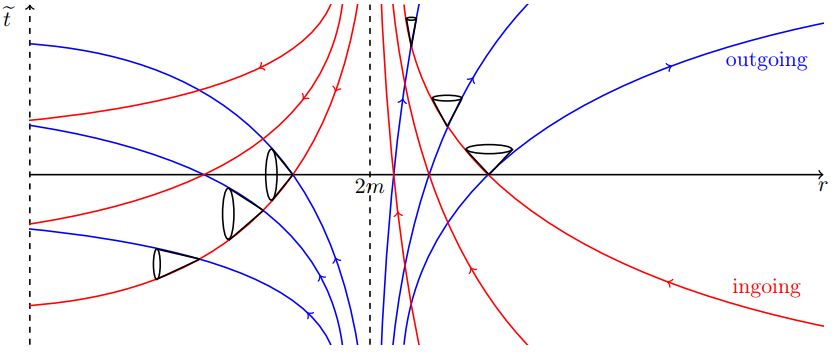
\includegraphics[width=0.9\textwidth]{Figuras/diag_schwc.png}
  \caption{diagrama de espaço-tempo em coordenadas de Schwartzchild - \textit{outgoing} e
          \textit{ingoing} representam raios de luz se afastando, e se aproximando, respectivamente. \\Fonte: Schuller, Dadhley (2015, p. 130)\cite{schuller2015}}
  \label{fig:diag_schwc}
\end{figure}

Note a distorção sofrida pelos cones de luz ao se aproximarem e se afastarem do horizonte de eventos. Note também que
esse diagrama, representado com essas coordenadas, poderia nos levar à conclusão de que as geodésicas tipo luz \textit{ingoing} (indo em direção ao buraco negro)
nunca atravessariam o horizonte de eventos, o que parece estar longe da verdade. Contudo, isso é o que nós observaríamos ao ver um objeto cair num
buraco negro de Schwartzchild, nunca veríamos esse objeto cruzar o horizonte de eventos - chegaria num ponto em que
ele aparecia \enquote{parado} em relação a nós, observadores, mas puramente devido a um fenômeno de dilatação
temporal extrema\footnote{como pode ser visto pelo lado esquerdo da equação (\ref{eq:dilat_temporal}) à medida que se toma $r \to 2GM^{+}$.}.  

Além de tudo isso, o diagrama $(t,r)$ nas coordenadas de Schwartzchild também pode nos levar a crer que a singularidade
$r=0$ é uma posição no espaço a ser alcançada, quando na verdade, veremos que se trata mais de uma \enquote{posição no tempo}\footnote{Tecnicamente, dizemos que a coordenada radial se torna tipo tempo, ou \textit{timelike}, que pode ser visualizada na figura \ref{fig:diag_schwc} pela \enquote{inversão} de direção dos cones de luz.},
a qual é impossível de ser evitada para objetos e feixes de luz que já cruzaram o horizonte de eventos.

Em geral, alguns dos problemas encontrados em diagramas $(t,r)$ com coordenadas de Schwartzschild são resolvidos puramente por uma
escolha melhor de coordenadas, podendo ainda manter a forma cartesiana do diagrama. Contudo, só conseguimos uma boa descrição \textit{global} e compacta da estrutura causal por meio dos Diagramas de Carter-Penrose, como pretendemos mostrar nas próximas sessões deste trabalho. Mas para construir esses diagramas, precisamos primeiro introduzir coordenadas que resolvem os problemas encontrados nas de Schwartzchild.
\section{Coordenadas de Kruskal-Szekeres}
Uma possível escolha de coordenadas que resolve os principais problemas encontrados com as coordenadas
de Schwartzchild, é a das coordenadas de Kruskal-Szekeres (K-S). Esse novo conjunto de coordenadas apresenta
duas propriedades importantes, a saber:
\begin{enumerate}[label=\arabic*., leftmargin=2.5em]
  \item Mantém os cones de luz inalterados com uma abertura interna de 90\degree.
  \item Não apresenta divergência em $r = 2GM$.
\end{enumerate}
Para construir as coordenadas de K-S, primeiro precisamos introduzir as coordenadas nulas\footnote{Nulas, pois, segue de suas definições que, curvas com $u=cte$ ou $v=cte$ são geodésicas do tipo luz descritas nas coordenadas tipo tempo e tipo espaço que as constroem.} $u$ e $v$:
%
\[
\left\{\;
\begin{aligned}
    u &\coloneq t - r_\star\\
    v &\coloneq t + r_\star
  \end{aligned}
\right.
\]
%
onde $r_\star$ é a \enquote{coordenada tartaruga}\footnoteB{O nome legal se deve ao fato de que $\dv*{r}{r_\star} \to 0$ à medida que se varia $r_\star$
em $r \to 2GM$, como se estivéssemos chegando cada vez mais devagar no horizonte de eventos a partir de variações nessa nova coordenada.}, construída de modo que a métrica deixe de apresentar a singularidade de coordenada em $r = 2GM$. Sua expressão em termos da coordenada radial de Schwartzschild é:
\begin{equation*}
  r_\star = r + 2GM\log\qty|\frac{r}{2GM}-1|.
\end{equation*}
Note que essas novas coordenadas (aparentemente) já resolvem nossos problemas: (1) já descrevem raios de luz com inclinação $\pm$1 num diagrama $(t,r_\star)$, e (2) removem a singularidade de coordenadas em $r = 2GM$.
Contudo, expressando a métrica com essas novas coordenadas, pode-se mostrar que ela ainda é degenerada (ou seja, se anula) em $r = 2GM$.
Para corrigir isso, aplicamos uma nova transformação nessas coordenadas, obtendo ao final de algumas manipulações e redefinições:
\begin{align*}
T(t,r,\theta,\varphi) &\coloneq \qty(\frac{r}{2GM}-1)^{1/2} e^{r/4GM}\sinh(\frac{t}{4GM})\\
R(t,r,\theta,\varphi) &\coloneq \qty(\frac{r}{2GM}-1)^{1/2} e^{r/4GM}\cosh(\frac{t}{4GM})
\end{align*}
De modo que a métrica de Schwartzchild, expressa nessas coordenadas, fica:
\begin{align*}
ds^2 = &\underbrace{\frac{32G^3M^3}{r}e^{-r/2GM}}(-dT^2 + dR^2) + r^2d\Omega^2\\
&\text{Fator Conforme}
\end{align*}
essa é, por vezes, chamada de \enquote{métrica de Kruskal}, e descreve globalmente a geometria do espaço-tempo na presença de um buraco negro de Schwartzchild. Por conta desta última propriedade, também é dita como a \enquote{extensão máxima} da solução de Schwartzchild\footnote{Não entraremos em detalhes sobre o que essa \enquote{extensão} significa num tratamento mais rigoroso e preciso; num primeiro momento, basta entender que é uma propriedade das coordenadas escolhidas que permite uma descrição mais completa da variedade espaço-temporal.}. 
Para geodésicas nulas nessas novas coordenadas, mantendo $\theta$ e $\varphi$ fixos (i.e., $d\Omega = 0$), obtemos uma métrica \enquote{com cara de Minkowisky} multiplicada por um fator conforme.

Poderíamos mostrar aqui um diagrama $(T,R)$ nas coordenadas de Kruskal e discutir todos os resultados impressionantes que saem dessas coordenadas, uma vez que eliminamos os problemas encontrados nas coordenadas de Schwartzschild, e obtivemos expressão não degenerada para a métrica. Porém, como o intuito do trabalho é
explorar, de fato, os diagramas de Carter-Penrose, deixaremos para discutir esses resultados na \S4. Seguiremos agora para uma outra ferramenta importante para a construção dos diagramas de Carter-Penrose, as \textit{transformações conformes}.

\section{Transformações Conformes}

Um dos pilares dos diagramas de Carter-Penrose, e na verdade, onde reside o \textit{core}
da ideia principal desses diagramas, são as noções de \textbf{transformações conformes} e de \textbf{compactação}, que trataremos mais adiante.

Até onde estamos interessados aqui, uma transformação conforme é 
basicamente uma mudança na geometria (portanto, uma mudança da métrica) que mantenha a estrutura causal do espaço-tempo
inalterada. Partiremos agora para a definição matemática, e mais precisa do queremos dizer com isso.

\begin{definição}
(Transformação Conforme)\\\\
Uma \textit{transformação conforme} é um mapeamento de um espaço-tempo $(\mathcal{M},g)$
no espaço-tempo $(\mathcal{M},\tilde{g})$, dado por
\begin{equation*}
  \tilde{g}_{\mu\nu}(x) = \omega^2(x)g_{\mu\nu}(x)
\end{equation*}
com $\omega \in C^{\infty}(\mathcal{M})$, e tal que $\omega(x) \neq 0, \forall x \in \mathcal{M}$; onde $x$ representa o conjunto das coordenadas $x^{\mu}$ avaliado num certo ponto do espaço-tempo.
\begin{flushright}
  \qed
\end{flushright}
\end{definição}
Segue da condição $\omega^2(x)>0$ na definição de $\tilde{g}$, que curvas tipo tempo/luz/espaço sob a métrica $g_{\mu\nu}$ também o serão para a 
métrica conforme $\tilde{g}_{\mu\nu}$:
\begin{align*}
   \tilde{g}(u_{\gamma},u_{\gamma}) &< 0 \Longleftrightarrow  g(u_{\gamma},u_{\gamma}) < 0\\
   \tilde{g}(u_{\gamma},u_{\gamma}) &= 0 \Longleftrightarrow  g(u_{\gamma},u_{\gamma}) = 0\\
   \tilde{g}(u_{\gamma},u_{\gamma}) &> 0 \Longleftrightarrow  g(u_{\gamma},u_{\gamma}) > 0.
\end{align*}
Além disso, a segunda condição acima garante que geodésicas tipo luz sob uma métrica também o serão
para a outra métrica, o que não vale de modo geral para geodésicas tipo tempo/espaço sob $g$, pois elas não necessariamente são mapeadas em \textit{geodésicas} sob $\tilde{g}$.

É sobre essas 3 últimas expressões que queremos dizer com \enquote{transformações conformes preservam a estrutura causal do espaço-tempo}.
\section{\enquote{Receita} para Diagramas de Carter-Penrose}
%%% Gráfico do desmos (Schwarzschild): https://www.desmos.com/calculator/nrxvtlo9nl
Como já dito anteriormente, visualizações pictóricas não são necessárias para o entendimento de diferentes espaços-tempos,
afinal, todas as características da geometria daquela métrica podem ser extraídas dela.
Porém, apesar de não necessários, diagramas no geral são de extrema importância na construção
de uma intuição sólida sobre certos aspectos de alguma teoria, e nesse caso não é diferente:
os diagramas de Penrose são tentativas (e êxitos!) de representar espaços-tempos de forma tal
que a interpretação da estrutura causal seja visualmente aparente.

Surgem então duas perguntas importantes: 
\begin{itemize}
    \item [1)]Como representar espaços-tempos ``infinitos'' em folhas de papel finitas?
    \item [2)]Como permitir uma interpretação fácil da estrutura causal sendo que os cones de luz se ``deformam'' ao fazer uma mudança de coordenadas?
\end{itemize}
Vamos entender a intuição por trás das respostas dessas duas perguntas. Se quisermos representar algo infinito em uma folha de papel, teremos inevitavelmente de aplicar alguma transformação que mapeie conjuntos infinitos em conjuntos finitos; mas transformações desse tipo não são nada estranhas para nós pois existem diversas funções que, por exemplo, mapeiam conjuntos reais infinitos em conjuntos reais finitos, tal como as funções $\arctan(x)$, $\tanh(x)$ e a função sigmoide $\sigma(x):=1/(1+e^{-x})$, que, de forma informal, fazem os seguintes mapas:
\begin{align*}
    \arctan(\mathbb{R})&=\left(-\frac{\pi}{2}, \frac{\pi}{2}\right)\\
    \tanh(\mathbb{R})&=\left(-1, 1\right)\\
    \sigma(\mathbb{R})&=\left(0, 1\right)
\end{align*}

Esses mapas só são possíveis pois $\mathbb{R}$ e intervalos reais são conjuntos densos. Com isso, vemos, portanto, a necessidade de aplicar uma transformação como esta, chamada intuitivamente de \textbf{compactificação}, ao construir um diagrama de Penrose. Porém, não podemos realizar uma compactificação das coordenadas sem que os cones de luz se deformem e compliquem uma análise da estrutura causal, para exemplificar isso, vamos aplicar ingenuamente uma dessas transformações no espaço plano de Minkowski e ver o resultado final. Comecemos então com o espaço de Minkowski em coordenadas esféricas:
\[g = -dt^2+dr^2+r^2d\Omega^2\]
Vamos compactificar apenas as coordenadas $r$ e $t$, transformando-as em $\bar{r}$ e $\bar{t}$ usando a função arco tangente tal que:
\[\bar{r}=\arctan(r),\quad\bar{t}=\arctan(t),\quad\bar{\Omega}=\Omega\]
Notemos que agora as coordenadas novas tiveram seus intervalos alterados: $\bar{r}\in(0,\pi/2)$ e $\bar{t}\in(-\pi/2,\pi/2)$. A métrica nessas coordenadas novas $g_{\mu'\!\nu'}$ é dada pela transformação da métrica antiga de acordo com a matriz jacobiana da transformação:
\[g_{\mu'\!\nu'}=\frac{dx^\mu}{dx^{\mu'}}\frac{dx^\nu}{dx^{\nu'}}g_{\mu\nu}\implies ds^2=-\sec^4(\bar{t})d\bar{t}^2+\sec^4(\bar{r})d\bar{r}^2 + \tan^2(\bar{r})d\bar{\Omega}^2\]
Vamos agora investigar os cones de luz: analisemos então as geodésicas tipo luz radiais. Geodésicas tipo luz nos dizem que $ds^2=0$, radiais nos indica que $d\bar{\theta}=d\bar{\phi}=0$ (ou seja $d\bar{\Omega}=0$), portanto:
\begin{equation}\sec^4(\bar{t})d\bar{t}^2=\sec^4(\bar{r})d\bar{r}^2\implies\tan(\bar{t})=\pm\tan(\bar{r})+k
\label{eq:geodesica_compact_errada}
\end{equation}
Onde $k$ é uma constante. Vamos ver então como fica o gráfico $\bar{t}\times\bar{r}$ dessas geodésicas na Figura \ref{fig:Minkowski_errada}:

\begin{comment}
\begin{figure}[h]
    \centering
    \includegraphics[width=0.2\linewidth]{figuras/Minkowski_errada.png}
    \caption{Diagrama nas coordenadas compactificadas $\bar{t}\times\bar{r}$ das geodésicas tipo tempo radiais do espaço-tempo de Minkowski variando a constante $k$ da Equação (\ref{eq:geodesica_compact_errada}). Em azul temos os casos $+$ e em vermelho temos os casos $-$ da Equação (\ref{eq:geodesica_compact_errada}).}
    \label{fig:Minkowski_errada}
\end{figure}
\end{comment}
Na Figura \ref{fig:Minkowski_errada}, vemos claramente que os cones de luz se distorcem, o que não explicita a estrutura causal do espaço de Minkowski, que é extremamente simples. Mas o que deu errado aqui? Voltemos na Equação (\ref{eq:geodesica_compact_errada}) para explicar. Para $\bar{t}$ e $\bar{r}$ suficientemente perto de zero, podemos fazer a aproximação $\tan(x)\approx x$, assim, perto da origem, temos que:
\[\bar{t}=\pm\;\bar{r}+k\quad\text{(perto da origem)}\]
Que são os cones de luz que estamos acostumados (com abertura de noventa graus e se abrindo na direção de $\bar{t}$ crescente). Porém ao nos distanciarmos da origem, essa aproximação não é mais válida e começamos a observar a não linearidade da tangente, o que deforma os cones de luz para $k\neq 0$. Vemos então que a raiz desse problema não é a compactificação em si, mas sim as coordenadas que compactificamos: para enxergar isso, basta imaginar qual é a transformação de um ponto com $\bar{r}$ pequeno e $\bar{t}$ qualquer, dessa maneira, podemos usar a aproximação $\tan(\bar{r})\approx \bar{r}$ para $\bar{r}$, mas não para $\bar{t}$, ou seja, estamos compactificando as duas coordenadas de jeitos diferentes! Dessa forma, nesse caso, os cones de luz são ``amassados'' mais em uma direção ($\bar{t}$) do que outra ($\bar{r}$), o que, nesse caso, faz com que os cones de luz para $\bar{t}$ perto de $\pi/2$ se abram cada vez mais. A solução desse problema então seria compactificar as duas coordenadas não de forma independente, mas de forma à preservar os formatos dos cones de luz. Para isso, portanto, é necessário escolher coordenadas que apontam na direção dos cones de luz, pois assim não há como alterar seu formato.
\subsection{Aplicação em Schwartzchild}
Tomando as coordenadas de K-S para desecrever o espaço-tempo na presença de um buraco negro de Schwartzchild, escolhemos novas coordenadas nulas $U$ e $V$, e as relacionamos com $T$ e $R$ para escreveremos a métrica em termos das novas coordenadas nulas:
\[
\left\{\;
\begin{aligned}
    U &\coloneq T + R\\
    V &\coloneq T - R
  \end{aligned}
\right. \;\Rightarrow \; \left\{\;
\begin{aligned}
    T &= \frac{1}{2}(U+V)\\[0.75em]
    R &= \frac{1}{2}(U-V)
  \end{aligned}
\right. \Rightarrow \; \left\{\;
\begin{aligned}
    dT &= \frac{1}{2}(dU+dV)\\[0.75em]
    dR &= \frac{1}{2}(dU-dV).
  \end{aligned}
\right.
\]
Após poucas contas, a métrica fica descrita da seguinte forma:
\[ ds^2 = \frac{16GM}{r}e^{-r/2GM}(dUdV + dVdU).\]
Uma primeira análise da métrica confirma que geodésicas tipo luz são descritas por curvas $U=cte$ e $V=cte$, que num diagrama cartesiano $(T,R)$ corresponde a retas de inclinação $\pm 1$, como era desejado.

Aplicando agora uma compactificação, dada pelo mapeamento
\[ \tilde{U} = \arctan(U) \;\; \text{e} \;\; \tilde{V} = \arctan(V) \]
e prestando atenção nos domínios sobre os quais estão definidas as funções de coordenadas, podemos desenhar o diagrama de Carter-Penrose para a solução de Schwartzchild, expresso na figura \ref{fig:penrose_schwc}.b

\begin{figure}[h!]
    \centering
    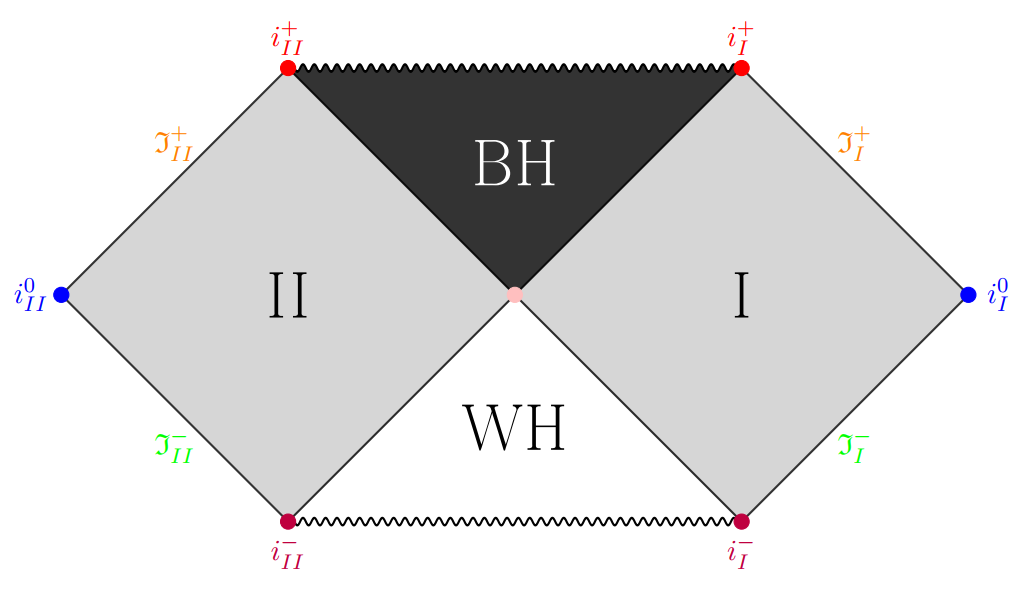
\includegraphics[width=1\linewidth]{Figuras/penrose_schwc.png}
    \caption{.}
    \label{fig:Minkowski_errada}
\end{figure}

\section{Conclusão}





% --- BIBLIOGRAFIA ---
\newpage
\nocite{*}
\printbibliography[title={Referências}]

\end{document}